%%% Laboratory	 Notes
%%% Template by Mikhail Klassen, April 2013
%%% Contributions from Sarah Mount, May 2014
\documentclass[a4paper]{tufte-handout}
\usepackage{tikz}

\newcommand{\workingDate}{\textsc{April $|$ 2022}}
\newcommand{\userName}{A.Belcaid}
\newcommand{\institution}{ENSA-Safi}

\usepackage{lab_notes}

\usepackage{hyperref}
\hypersetup{
    pdffitwindow=false,            % window fit to page
    pdfstartview={Fit},            % fits width of page to window
    pdftitle={Correction TD4},     % document title
    pdfauthor={A.Belcaid},         % author name
    pdfsubject={},                 % document topic(s)
    pdfnewwindow=true,             % links in new window
    colorlinks=true,               % coloured links, not boxed
    linkcolor=DarkScarletRed,      % colour of internal links
    citecolor=DarkChameleon,       % colour of links to bibliography
    filecolor=DarkPlum,            % colour of file links
    urlcolor=DarkSkyBlue           % colour of external links
}


\title{Solution TD 5}
\date{2022}

\begin{document}
\maketitle

\renewcommand{\P}{\mathbf{P}}

\section{Mots d'un alphabet}

\begin{enumerate}
  \item On dispose de $5$ choix pour la premiere lettre, $4$ pour la deuxieme.
    Ainsi le nombre de choix possible est 
      \begin{equation*}
       5 \times 4 \times \ldots \times 1  = 5! = 60 
      \end{equation*}
      
    \item Le nombre de sous ensembles est donne par : 
      \begin{equation*}
         2^5 = 32 
      \end{equation*}
    \item On applique le principe de denomrement avec trois scenarios:
      \begin{enumerate}
        \item Tout d'abord on choisit si $A$ va precedder $B$ ou non, alors on
          $\mathbf{2}$ choix.
        \item Ensuite, on dois choisir la position du couple $AB$ ( ou $BA$)
          dans le mot. On dipose alors de $\mathbf{4}$ choix.\footnote{Ces
          positions sont soit 1,2,3 ou 4}.
        \item Finalement pour chaque emplacement du couple $AB$, il nous faut
          placer le reste des trois lettres. Ceci est donne par le nombre de
          permutation de l'ensemble $\{C,D,E\}$. On trouve alors $3! = 6$
      \end{enumerate}
      Ainsi le nombre ces motes sera donne par:
      \begin{equation*}
       2\cdot 4 \cdot 6 = 48 
      \end{equation*}
    \item Le cardinal de l'espace d'etats est 
      $$
      card(\Omega) = 5! = 120
      $$
      Ainsi, la probabilite de construire un tel mot est:

      $$
      \P(A) = \dfrac{48}{120} = \dfrac{2}{5} = 0.4
      $$
\end{enumerate}


\section{Anecdode Anniversaire}

On cherche a calculer la probabilite  de $A = \{\text{\small aucun anniversaire conside
avec les autres}\}$.\\

On pose alors l'espace des etats 

\begin{eqnarray*}
  \Omega &= & \{\text{toutes les anniversaires possible}\}\\
  card\{\Omega\} &=& (365)^n
\end{eqnarray*}

Pour l'evenement d'interet, on dispose alors de 

$$
365\cdot 364\cdot 363\cdot \ldots (365 - n + 1)
$$

On obtient alors
\begin{equation*}
  \P(A) = \dfrac{365\cdot 364 \cdot \ldots (365 - n + 1)  }{(365)^n} 
\end{equation*}

\begin{marginfigure}
   \centering
   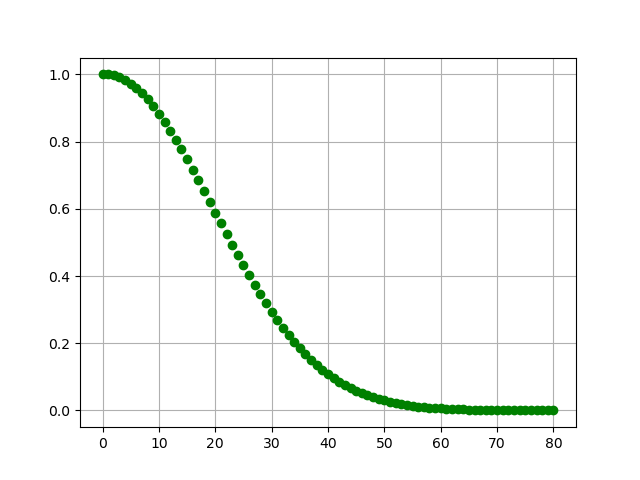
\includegraphics[width=0.8\textwidth]{./birthday.png}
   \caption{Convergene rapide de cette probbailite vers 0}
   \label{fig:birth}
\end{marginfigure}

l'anecdote ici est que ce nombre converge facilement vers $\mathbf{0}$ comme le
montre la figure (\ref{fig:birth}). Ainsi deja pour une fete de $n = 40$ personnes on a une
probbabilite de $\P =\mathbf{0.10} $.

\section{Probleme des tours}

On note l'evenement $A = \{\text{\small toutes les tours ne s'attaquent pas}\}$

On alors:

$$
\P (A) = \frac{\vert \text{Position correcte des tours}\vert}{\vert\text{Toutes
les positions possibles.} \vert}
$$

Pour le cardinal de toutes les positions possibles on obtient:

$$
64\cdot 63 \cdot \ldots\cdot 57
$$

Pour la deuxieme quantite, on doit placer sequentiellement $8$ tours. Ainsi
\begin{itemize}
  \item Pour la premiere tour on dispose de $$64= 8 \times 8$$ cases
    disponibles.\footnote{Tout l'echequier est disponible}.
  \item Pour la deuxieme tour choisir la la ligne $i$ et la colonne $j$ ou
    ($(i,j)$) est la position de la premiere tour. Ainsi on obtient $$49 = 7
    \times 7$$.
  \item Par la meme analyse on obtient 
    $6^2$ pour la troisieme, $5^2$ pour la quatrieme etc.
\end{itemize}

En resumant le cardinal d'evenement d'interet est 
$$
8^2 \cdot 7^2 \cdot \ldots  4 . 1 = \prod_{i=1}^8 i^2
$$

Finalement la proabilite est donnee par:

$$
\P(A) = \dfrac{\prod_{i=1}^8 i^2}{64\cdot 63\cdot \ldots 57}
$$
\end{document}

